\documentclass{article}

\usepackage[margin=1in]{geometry}

\usepackage[colorlinks]{hyperref}
\usepackage{biblatex}
\addbibresource{references.bib}

\usepackage{authblk}
\usepackage{graphicx}
\usepackage{amsthm}
\usepackage{amssymb}
\usepackage{amsmath}
\usepackage{enumerate}
\usepackage{caption}
\usepackage{subcaption}
\usepackage{multicol}
\usepackage{listings}
% \usepackage{newpxtext,newpxmath}

\theoremstyle{definition}
\newtheorem{theorem}{Theorem}%[section]
\newtheorem{lemma}[theorem]{Lemma}
\newtheorem{proposition}[theorem]{Proposition}
\newtheorem{definition}[theorem]{Definition}
\newtheorem{remark}[theorem]{Remark}
\newtheorem{conjecture}[theorem]{Conjecture}
\numberwithin{equation}{section}

\title{Bistable periodic traveling waves and dynamical stabilization in an integrodifference equation with strong Allee effect and overcompensatory cycles}
%\author[1]{Bingtuan Li}
\author{Michael Nestor}
%\author{}%Michael Nestor (mdnest01@gmail.com)}
%\affil[1]{Department of Mathematics, University of Louisville}
%\date{}

\begin{document}

\maketitle

\tableofcontents

\section{Introduction}

In this study we consider the integrodifference equation
\begin{equation}
u_{t+1}(x) = Qu_t(x)=\int_{-\infty}^{\infty} k(x-z) \, g(u_t(z)) \, dz \label{ide}
\end{equation}
when the growth function $g$ exhibits both strong Allee effect (stability at zero) and overcompensation (non-monotonicity at carrying capacity) leading to periodic cycles.
We consider the following two-parameter growth function
\begin{equation} \label{g}
g(u;a,r)=u\exp(r(1-u)(\frac{u}{a}-1))
\end{equation}
where $r \geq 0$ is a growth rate parameter and $a \in (0,1]$ is an Allee threshold.
The dispersal kernel $k$ is generally taken to be a symmetric probability density; in applications it is typically given by the Laplace or Gaussian distribution.
We focus specifically on traveling wave solutions, which are important for modeling biological invasions and represent the limiting behavior of solutions started from a bounded domain.

This model represents a combination of two effects which have previously been studied independently:
\begin{itemize}
\item monotone growth models with an Allee threshold exhibit bistable traveling waves with a unique propagation speed determined by the growth function alone (and not the kernel); a recent proof was given in \cite{LO22},
\item non-monotone (overcompensatory) growth models with stable cycles but without an Allee threshold exhibit complex phenomena like period-doubling wave fronts stacked wave-trains, wherein the leading invasion wave is trailed by one or more periodic traveling waves of lesser speeds. Furthermore, the separating wave fronts leave in between them a growing plateau on which the solution takes an unstable equilibrium value in a phenomenon known as {\it dynamical stabilization}; the equilibrium is said to be {\it dynamically stabilized} by the dispersal. These were originally observed in \cite{K92} and more recent analytical work was done in \cite{BLL20}, \cite{BLL18}.
\end{itemize}

The combinations of these effects has been studied in integrodifference equations; numerically in \cite{SLMNS17} and simplified piecewise growth models analytically in \cite{O17} and \cite{NL22}. TODO: More info.

Our main contribution here is a primarily numerical investigation of traveling wave behavior in this model.
Specifically, the following phenomenon which, to our knowledge, has not been described before in integrodifference models: the existence of a {\it periodic bistable wave} directly connecting the stable cycle to zero.
We conjecture this wave exists precisely when the trailing wave connecting the stable cycle to one overtakes the leading wave connecting the carrying capacity to zero in speed.
This behavior is depicted in \autoref{fig:fig1} for the case when the growth function has a stable $2$-cycle $\{u^+,u^-\}$

\begin{figure}[htbp]
    \centering
    \begin{subfigure}{0.5\textwidth}
        %\centering
        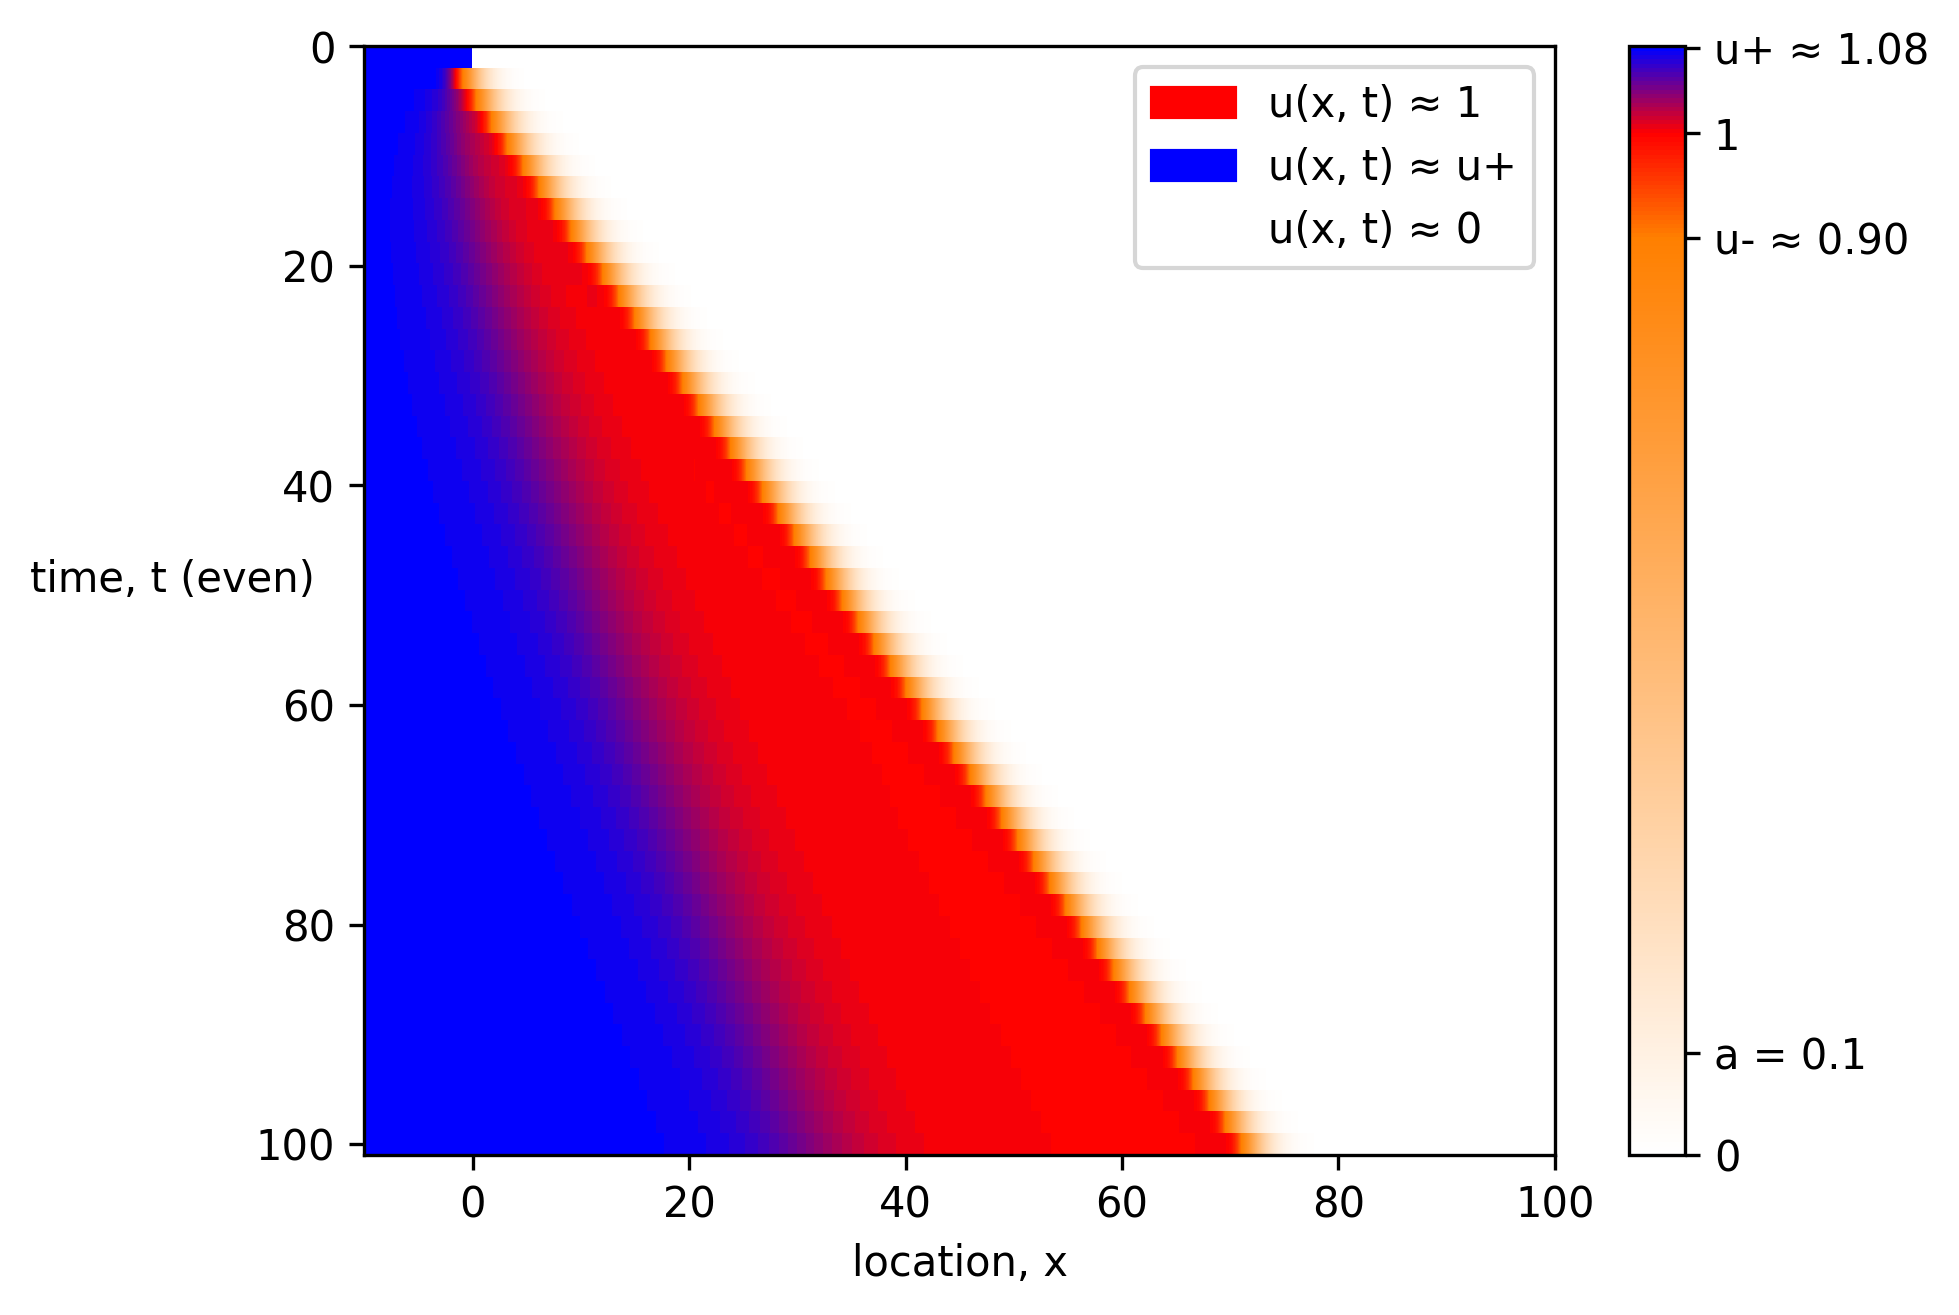
\includegraphics[width=\linewidth]{figures/example_spacetime0.png}
        %\caption{First subcaption.}
        \label{fig:fig1}
    \end{subfigure}\hfill
    \begin{subfigure}{0.5\textwidth}
        %\centering
        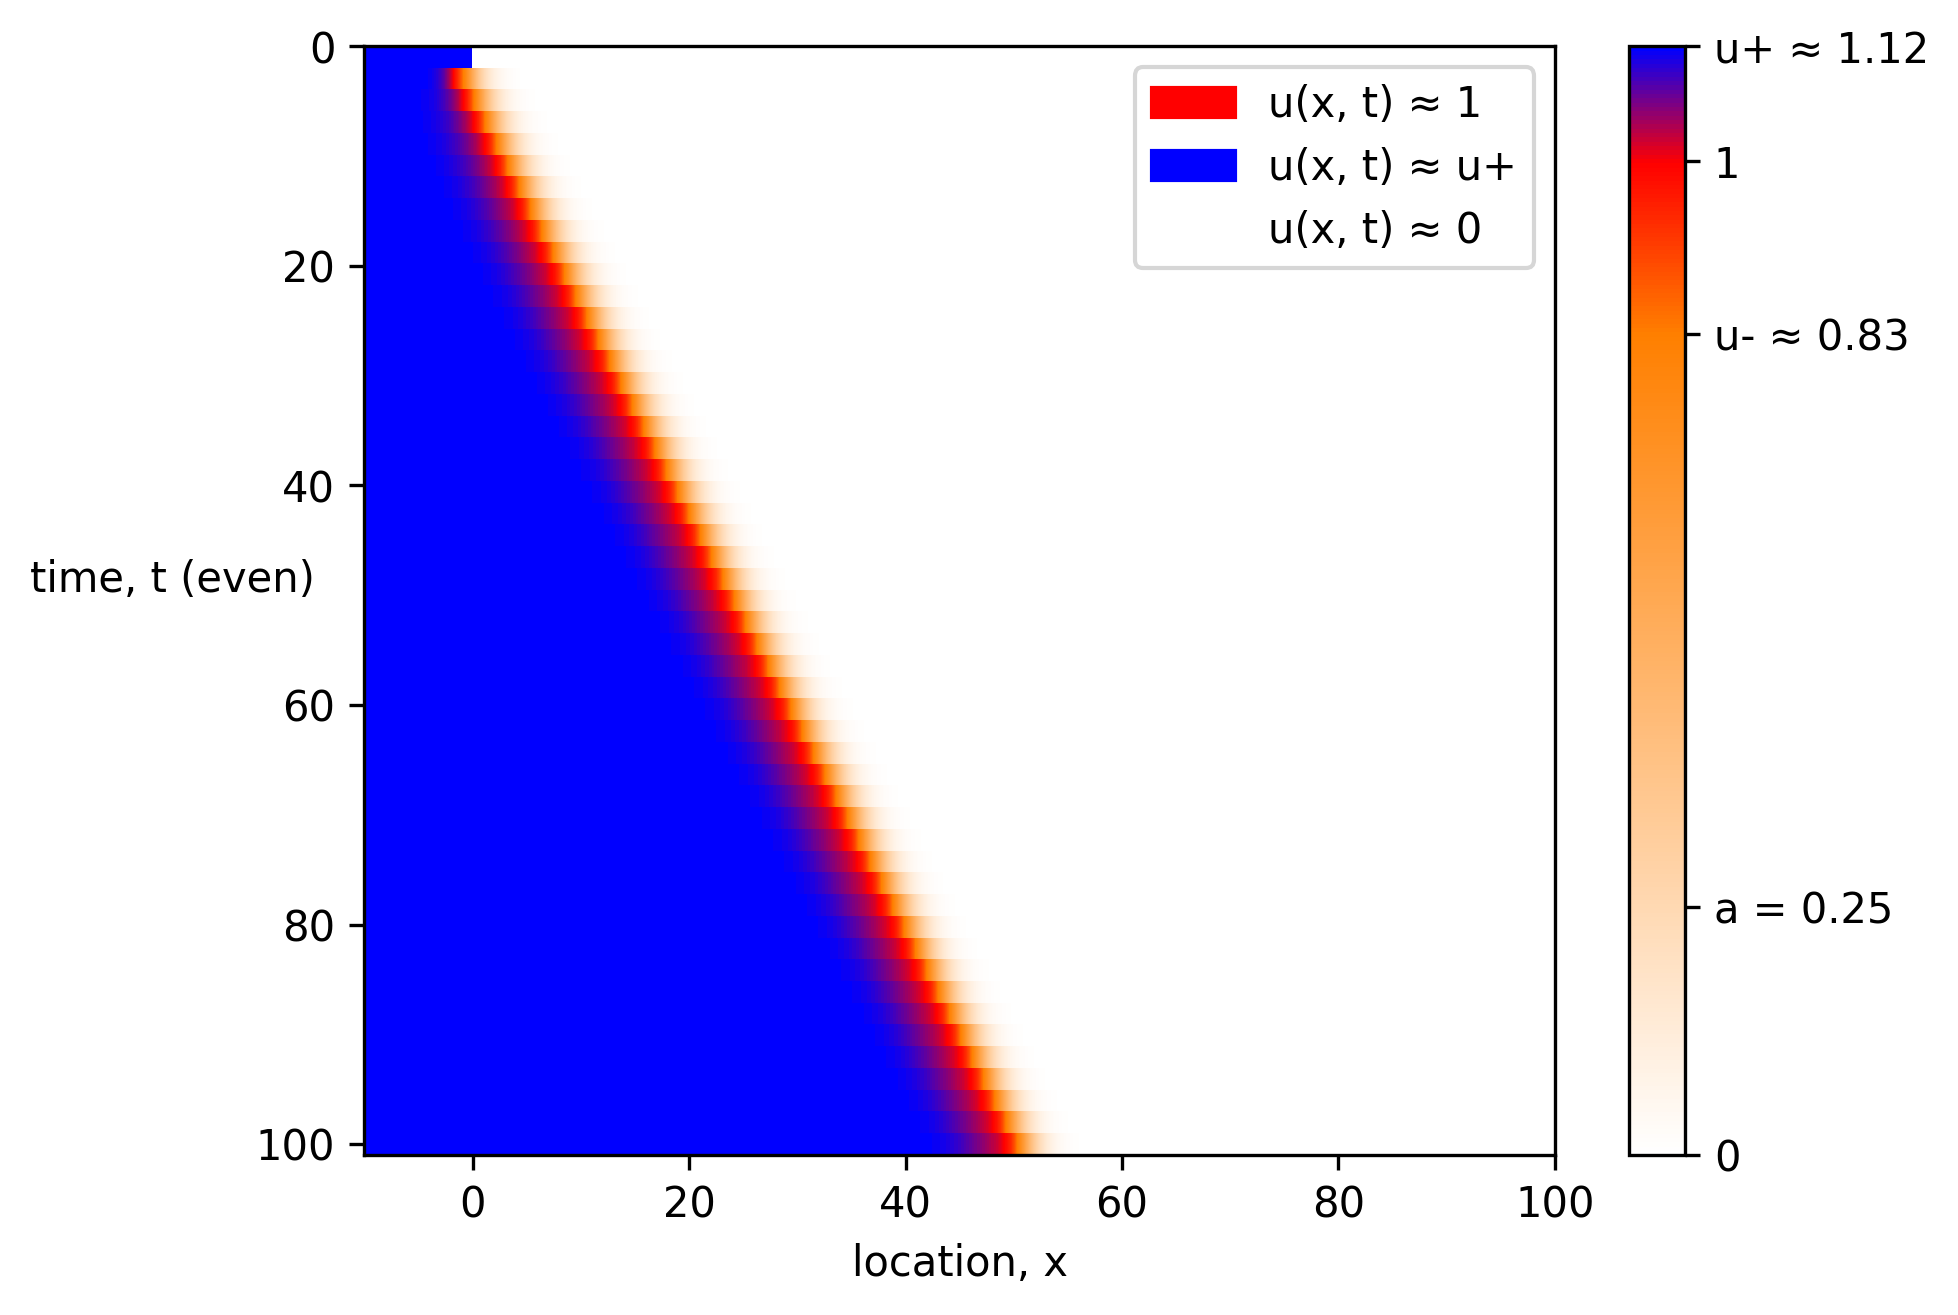
\includegraphics[width=\linewidth]{figures/example_spacetime1.png}
        %\caption{Second subcaption.}
        \label{fig:fig2}
    \end{subfigure}
    \caption{Two distinct outcomes from step initial data connecting $u=u^+$ to $u=0$ plotted on even time steps $t \in \{0,2,4,...\}$. Left: with $a=0.1$, $r=0.23$, the solution converges to a stacked wave train consisting of a monostable $2$-periodic traveling wave connecting $\{u^+,u^-\}$ to $1$ followed by a monostable traveling wave connecting $1$ to $0$. Right: with $a=0.25$, $r=0.75$, the solution converges to a bistable periodic traveling wave directly connecting $\{u^+,u^-\}$ to $0$.}
    \label{fig:fig1}
\end{figure}



\section{Analysis}

\subsection{Local growth dynamics}

This section contains basic facts about the growth function \eqref{g}.
%$$ g(u;a,r)=u\exp(r(1-u)(\frac{u}{a}-1)) $$
%Desmos plot of graph: \href{https://www.desmos.com/calculator/bm9fvoluqx}{https://www.desmos.com/calculator/bm9fvoluqx}


\begin{figure}[htbp]
    \centering
    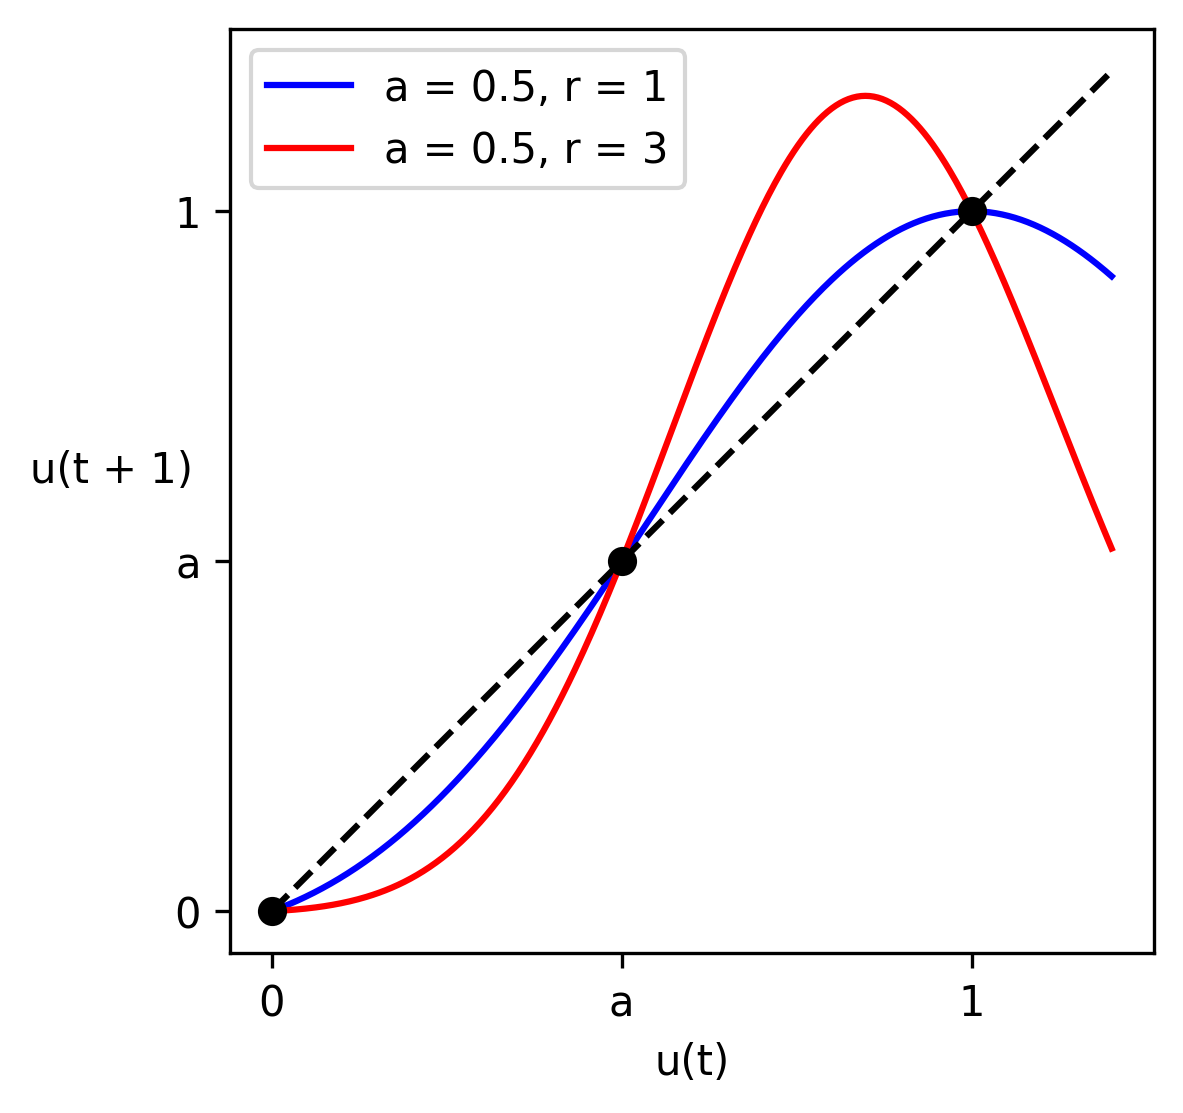
\includegraphics[width=0.5\textwidth]{figures/growthmap.png}
    \caption{The growth map with a couple different choices of parameters.}
    \label{fig:example}
\end{figure}

\begin{proposition}
The growth function \eqref{g} has the following properties:
\begin{enumerate}[i.]
\item $g(0)=0$, $g(a)=a$, and $g(1)=1$ are the only fixed points.
\item $0<g(u)<u$ on $(0,a)\cup(1,\infty)$ and $g(u)>u$ on $(a,1)$.
\item $g$ is increasing on $[0,u^*]$ and decreasing on $[u^*,\infty)$ where $u^*$ is the global maximum given by
$$u^* = \frac{1}{4}\left(a+1+\sqrt{(a+1)^2+\frac{8a}{r}}\right) $$
\item $g$ is monotone on $[0,1]$ iff. $\displaystyle r \leq \frac{a}{a-1}$.
\item $0<g'(0)<1$, making $u=0$ an asymptotically stable fixed point.
\item $g'(a)>1$,
\item TODO: more here
\end{enumerate}
\end{proposition}

\subsection{Traveling waves}

In this section, we describe the traveling waves we are interested in.

A traveling wave connecting $1$ to $0$, which is bistable when $r<r_1$ and monostable when $r>r_1$:
\begin{equation} \tag{TW}
Qw_1(x)=w_1(x-c_1), \quad w_1(-\infty)=1, \quad w_1(+\infty)=0 \label{eq}
\end{equation}

When $\{u^+,u^-\}$ form a stable $2$-cycle, a monostable $2$-periodic wave connecting $u^\pm$ to $1$:
\begin{equation} \tag{MPTW}
Q^2w_2(x)=w_2(x-2c_2), \quad w_2(-\infty)=u^+, \quad w_2(+\infty)=1
\end{equation}

When $\{u^+,u^-\}$ form a stable $2$-cycle, a bistable $2$-periodic wave connecting $u^\pm$ directly to $0$:
\begin{equation} \tag{BPTW}
Q^2w(x)=w(x-2c), \quad w(-\infty)=u^+, \quad w(+\infty)=0
\end{equation}


\subsection{Initial value problems}

We are also interested in the following initial value problems, both when $r_1 < r < r_2$:

With step initial data:
\begin{equation} \tag{IVP}
\begin{aligned}
u_{t+1} &= Qu_t \\
u_0(x) &= \begin{cases} u^+ & x \leq 0 \\ 0 & u > 0 \end{cases}
\end{aligned}
\end{equation}
and with compact initial data on an interval of radius $R>0$:
\begin{equation} \tag{IVP}
\begin{aligned}
u_{t+1} &= Qu_t \\
u_0(x) &= \begin{cases} u^+ & |x| \leq R \\ 0 & |x| > R \end{cases}
\end{aligned}
\end{equation}

% \subsection{Definitions}

% We will alternatively refer to periodic traveling wave (PTW) solutions vs profiles.
% \begin{itemize}
% \item A PTW solution is a sequence $u_t(x)$ satisfying $u_{t+p}(x-cp)$
% \end{itemize}

% For convenience; TODO: remove later.

% \begin{enumerate}
% \item A sequence $u_t(x)$ is called a traveling wave solution with velocity $c$ if $u_{t+1}(x)=u_t(x-c)$.
% \item Equivalently, a traveling wave can be written as $u_t(x)=w(x-ct)$ where $w$ is called the traveling wave profile, satisfying $Qw(x)=w(x-c)$ and $w(\pm\infty)=\ell^\pm$.
% \item It is called a traveling front connecting $\ell^-$ to $\ell^+$ if we add the conditions $u_t(\pm\infty)=\pm\ell$, where necessarily $\ell\pm$ are fixed points of $g$.
% \item $u_t$ is called a periodic traveling wave with period $p$ connecting $\ell^-$ to $\ell^+$ with mean velocity $c$ if $u_{t+p}(x)=u_t(x-cp)$ and $u_t(\pm\infty)=g^t(\ell\infty)$, where necessarily $\ell^\pm$ are $p$-periodic points of $g$.
% \item Equivalently, a periodic traveling wave can be written as $u_t(x)=w_t(x-ct)$ where $w_t$ is called the periodic traveling wave profile, satisfying $Q^pw(x)=w(x-cp)$ and $w_t(\pm\infty)=g^t(\ell^\pm)$.
% \end{enumerate}

% \begin{itemize}
% \item Every PTW solution is a TW solution with $p=1$.
% \item Every PTW profile $w_t$ is a TW profile with $w_t$ constant in $t$. 
% \item If $w_t$ is a PTW profile then $w_{t+p}=w_t$.
% \end{itemize}


\subsection{Case 1: monotone growth}

When the growth function is monotone, we can apply the results of \cite{LO22} to obtain the existence of a traveling wave with a unique propagation speed. The following is an immediate application of Theorem 3.1 in \cite{LO22}:

\begin{proposition}
Suppose $r\leq r_m$.
Then there exists a unique $c_1^*$ such that there exists a nonincreasing traveling wave $w_1 \in C(\mathbb{R},[0,1])$ such that
$$ Qw_1(x)=w_1(x-c_1^*), \quad w_1(-\infty)=1, \quad w_1(+\infty)=0 $$
\end{proposition}

\subsection{Case 2: nonmonotone growth, stable carrying capacity}

\subsection{Case 3: nonmonotone growth, stable 2-cycles}

When $r_1 < r < r_m^1$ we can apply the results of Theorem 3.1 in \cite{BLL18}:

\begin{proposition}
Suppose $r_1 < r \leq r_m^1$ (so that $g^2$ is monotone on $[u^-,u^+]$). Then there exists a {\it spreading speed} $c_2^*$ for the double-iterate operator $Q^2$ from $1$ to $u^+$. This means:
\begin{enumerate}
\item for any initial data $u_0 \in C(\mathbb{R},[1,u^+])$ with $u_0(x)=1$ outside a compact set, then
$$ \lim_{t\to\infty} \sup_{|x| \geq ct} Q^{2t} u_0(x) = 1, \quad \forall c > c_2^* $$
\item for any initial data $u_0 \neq 1$,
$$ \lim_{t\to\infty} \inf_{|x| \leq ct} Q^{2t}u_0(x) = u^+, \quad \forall c \in (0,c_2^*) $$
\end{enumerate}
\end{proposition}

We also get the existence of traveling waves from Theorem 3.2 in \cite{BLL18}:

\begin{proposition}
If $r_1 < r \leq r_m^1$, then with $c_2^*$ given in the previous theorem, there exists a monotone traveling wave solution $u_{2t}(x)=w_2(x-2c_2^*t)$ such that $w_3(-\infty)=u^+$ and $w_2(+\infty)=1$.
\end{proposition}

TODO: more here?


\subsection{Else: nonmonotone growth, higher cycles and chaos}

\section{Numerical simulations and conjectures}

\subsection{The initial value problem with step initial data connecting $u^+$ to $0$}

In this section we consider the initial value problem
\begin{equation} \label{ivp} \begin{aligned}
u_0(x) &= \begin{cases} u^+ & x \leq 0 \\ 0 & x > 0 \end{cases} \\
u_{t+1}(x) &= Qu_t(x)
\end{aligned} \end{equation}
when the growth function has a stable $2$-cycle, i.e. when $r_1(a) < r < r_2(a)$.
Our basic observation, as depicted in \autoref{fig:fig1}, is that depending on the choice of parameters, the solution converges either to a 2-periodic {\it bistable wave} directly connecting $u^+$ to $0$, or a pair of {\it stacked waves} moving at different velocities connecting $u^+$ to $1$ and $1$ to $0$ respectively.

We make this prediction precise in the following conjecture:
\begin{conjecture}
The solution $u_t(x)$ to the initial value problem \eqref{ivp} falls in one of two cases depending on the growth parameters $(a, r)$:
\begin{itemize}
\item Case 1 (stacked wave): the solution converges uniformly to a superposition of traveling waves, that is
$$ \sup_{x \in \mathbb{R}}\|u_{2t}(x)-w_1(x - 2c_1t)-w_2(x- 2c_2t)+1\|_\infty \to 0 $$
where $w_1$ is a solution to \eqref{w1} and $w_2$ is a solution to \eqref{w2}.
\item Case 2 (bistable wave): the solution converges uniformly to a bistable traveling wave, that is
$$ \sup_{x \in \mathbb{R}}\|u_{2t}(x)-w(x - 2c_2t)\|_\infty \to 0 $$
where $w$ is a solution to \eqref{w}
\end{itemize}
\end{conjecture}

\begin{remark}
Notice that our characterization of stacked waves only requires uniform convergence on compact sets.
\end{remark}



% \begin{enumerate}
% \item $w_0(-\infty)=u^+$,
% \item $w_0(+\infty)=0$,
% \item $Q^2w_t(x)=w_t(x-2c)$,
% \item $w_{t+2}=w_t$.
% \end{enumerate}
% \item converges to a pair of stacked traveling waves, TODO: explain
% \end{enumerate}

Based on this conjecture, we can design a numerical experiment to estimate the wave speeds in either case.
Attach to the solution the following sequence of front-tracking points, for a given $\epsilon>0$:
$$ \alpha_t = \sup \{ x \mid |u_t(x) - g^t(u^+)| \geq \epsilon \}, \quad \beta_t = \inf \{ x \mid |u_t(x)| \geq \epsilon \} $$

and the wave speed estimates
$$ c_2(t)=\frac{1}{2}(\alpha_{t+2}-\alpha_t), \quad c_1(t)=\beta_{t+1}-\beta_t $$



Our next plot is based on the following observation:
$$ \lim_{t\to\infty}c_t^+(u^+,\epsilon)-c_t^-(0,\epsilon) = \begin{cases}
0 & \text{in case 1} \\
c_1-c_2 & \text{in case 2}
\end{cases} $$
\autoref{fig:cdiff} shows the result of approximating the above limit for a range of $(a, r)$ values.
We observe that both behaviors occur on a nontrivial region of parameter space.

A couple more conjectures to organize: (TODO)

\begin{conjecture}
Suppose 
\end{conjecture}

\begin{conjecture}
For sufficiently small $a \in (0,1)$ there exists a threshold $r_{thres}(a) \in (r_1(a),r_2(a))$ below which case 2 occurs, and above which case 1 occurs.
\end{conjecture}

% $$ \alpha_t(\epsilon) = \sup\{ x \mid |u_{2t}(x) - u^+| \geq \epsilon \}$$
% and
% $$ \beta_t(\epsilon) = \inf\{ x \mid |u_{t}(x)| \geq \epsilon \}$$
% and defined
% $$ \tilde c_2(\epsilon) = \alpha_{t+1}(\epsilon)-\alpha_t(\epsilon),\quad \tilde c_1(\epsilon) = \beta_{t+1}(\epsilon)-\beta_t(\epsilon) $$
% \begin{proposition}
% If the solution falls into Case 1, then for sufficiently small $\epsilon$,
% $$ \lim_{t\to\infty}\tilde c_1(\epsilon)=\lim_{t\to\infty}\tilde c_2(\epsilon)=c $$
% Otherwise, if the solution falls into Case 2, assuming $\sup_x w_1(x) < u^+$ and $\inf_x w_2(x)>0$, then for sufficiently small $\epsilon$,
% $$ \lim_{t\to\infty} \tilde c_1(\epsilon)=c_1, \quad \lim_{t\to\infty}\tilde c_2(\epsilon)=c_2 $$
% \end{proposition}

% \begin{proof}
% TODO. Appendix?
% \end{proof}

% Based on these observations, we conducted a parameter sweep to estimate the difference $\tilde c_1 - \tilde c_2$.

\begin{figure}[htbp]
    \centering
    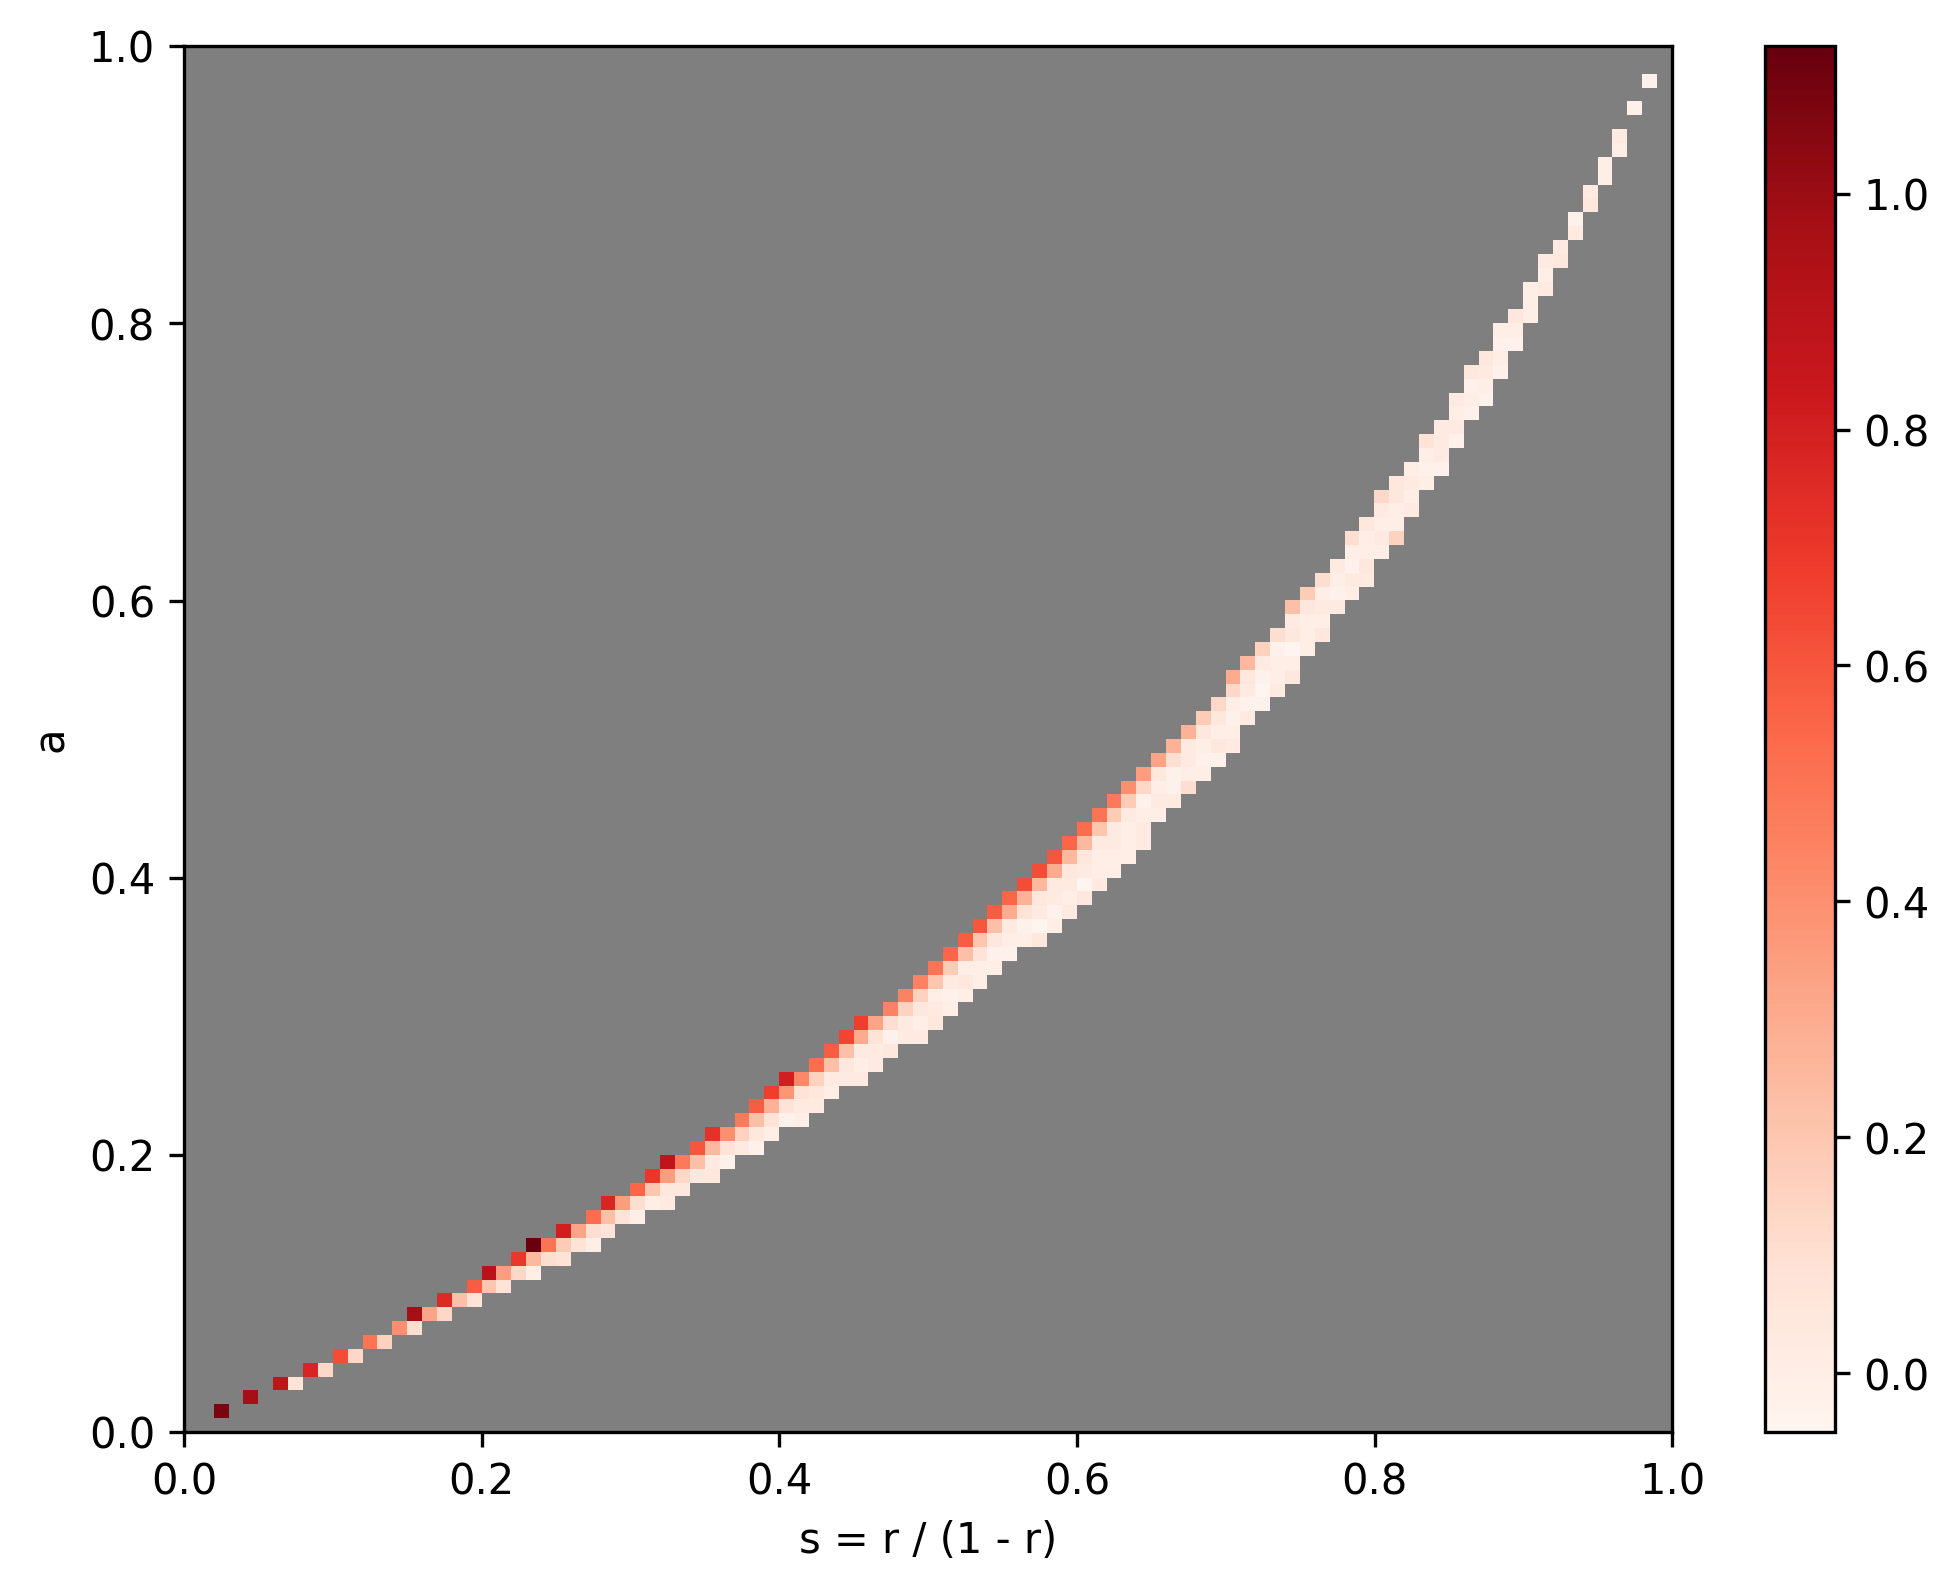
\includegraphics[width=0.5\textwidth]{figures/cdiff.png}
    %\caption{The growth map with a couple different choices of parameters.}
    \label{fig:cdiff}
\end{figure}

\subsection{Comparing wavespeeds via continuation method}

In the previous section, we conjectured two possible outcomes of the initial value problem \eqref{ivp} when $r_1(a) < r < r_2(a)$.
In the second case when two traveling waves emerged, our numerical algorithm allowed us to estimate both wave speeds.
In the first case however, when a bistable wave emerges, we gain no information about the existence of waves connecting $u^\pm$ to $1$ or $1$ to $0$.
For example, consider \autoref{fig:ivp2}, which depicts the initial value problem
\begin{equation} \label{ivp2}
\begin{aligned}
u_0(x) &= \begin{cases} 1 & x \leq 0 \\ 0 & x > 0 \end{cases} \\
u_{t+1}(x) &= Qu_t(x)
\end{aligned}
\end{equation}
with growth parameters $a=0.25$, $r=0.75$ (for which a bistable wave appears in problem \eqref{ivp}).
Rather than converge to a traveling wave connecting $1$ to $0$, the solution converges to a pair of outgoing waves, connecting $u^\pm$ to $1$ on the left and $u^\pm$ to $0$ on the right.

\begin{figure}[htbp]
    \centering
    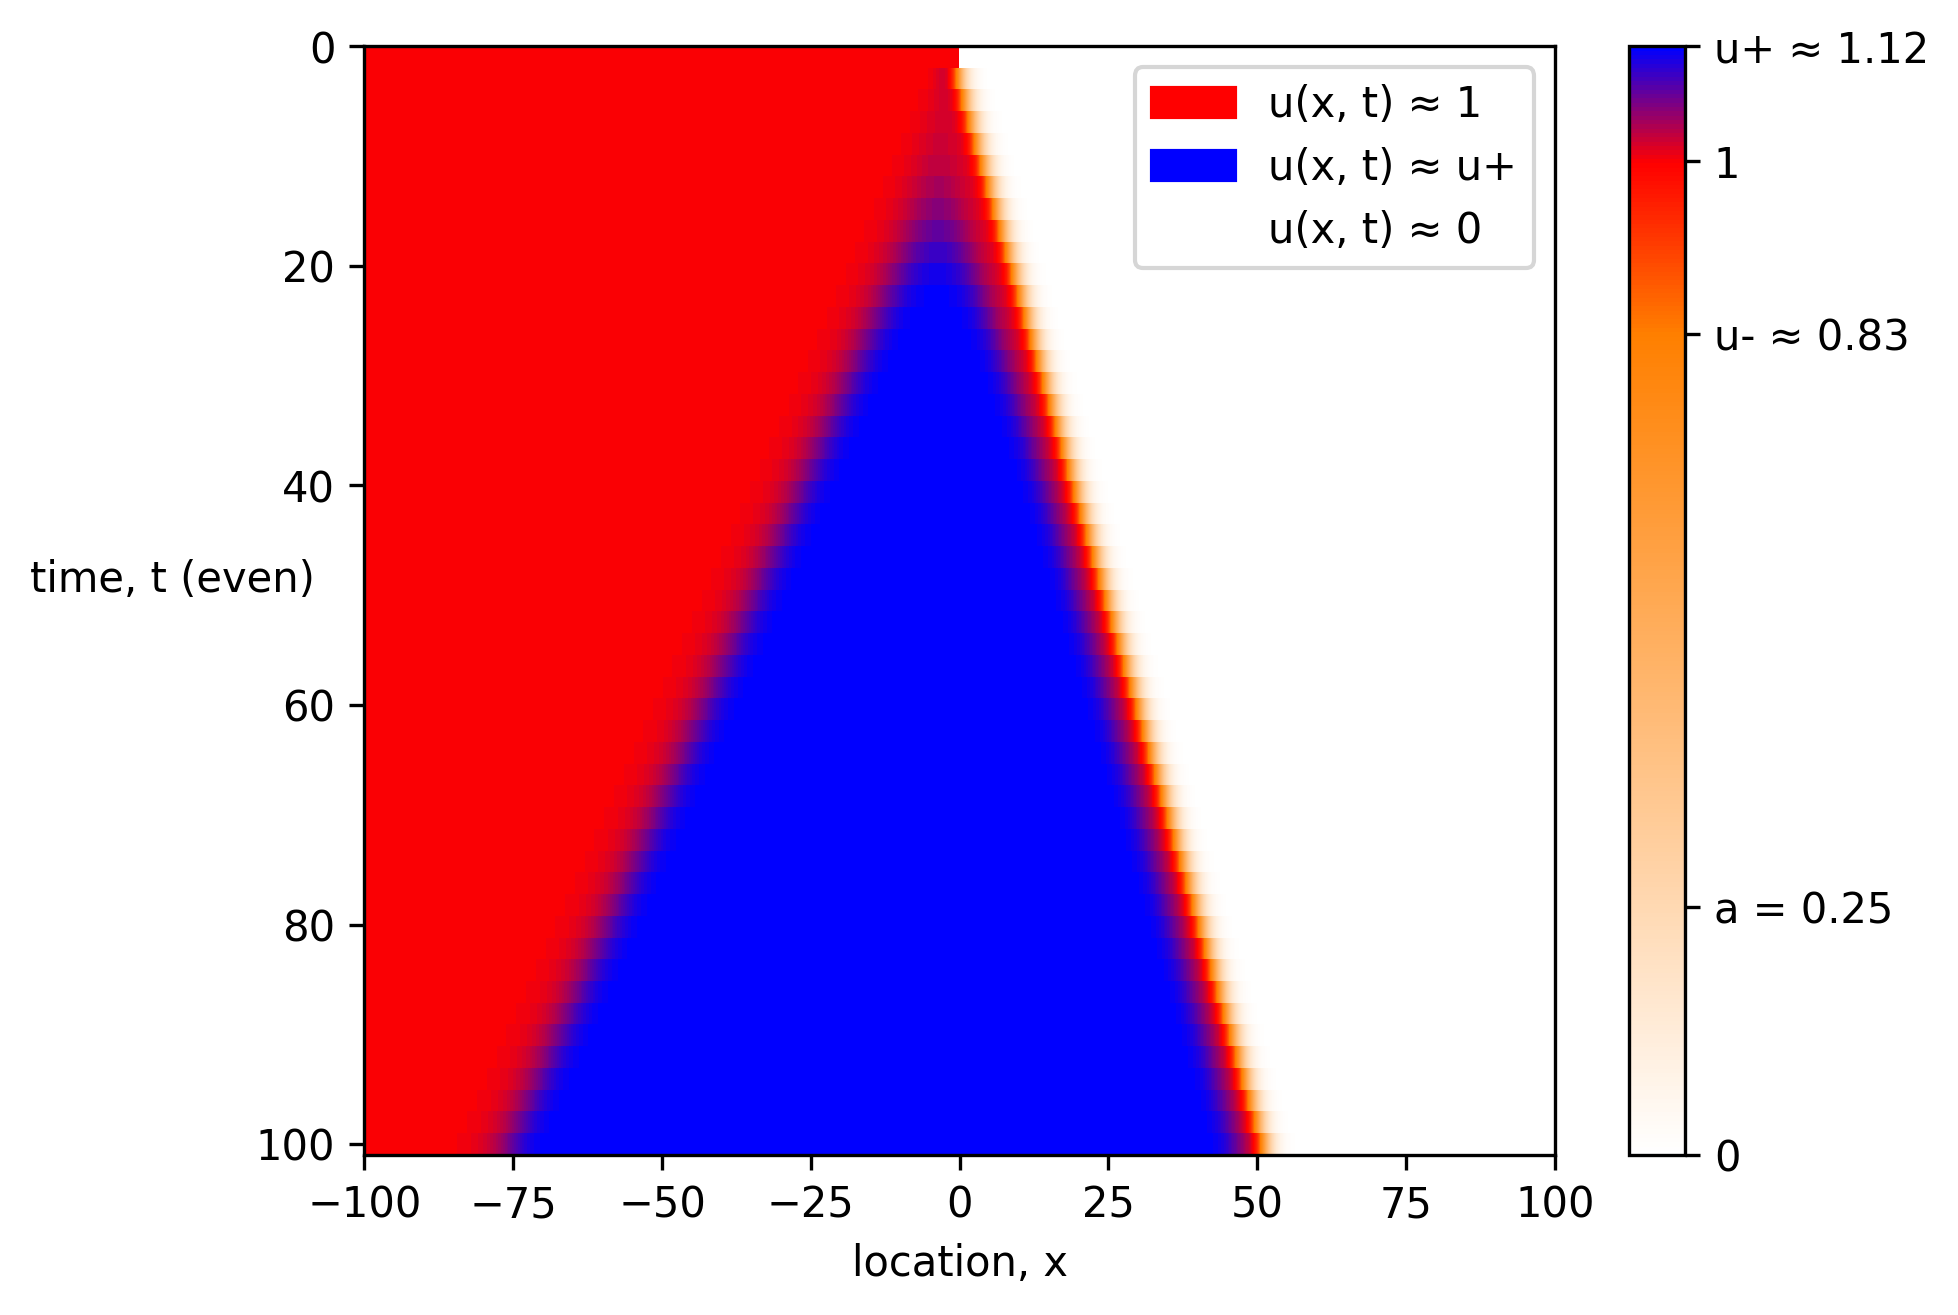
\includegraphics[width=0.5\textwidth]{figures/example_spacetime2.png}
    %\caption{The growth map with a couple different choices of parameters.}
    \label{fig:ivp2}
\end{figure}

Thus, if there is a wave connecting $1$ to $0$, we are unable to observe it from the initial value problem.
Instead, we consider a continuation method as follows which slowly increases the growth rate parameter $r$ from the starting value $r_m(a)$, at which the growth function is monotone and a $(1,0)$ wave exists by theorem, and slowly increases to the value we are interested in.

Specifically we set up the following problem for a given $(r,a)$ such that $r_1(a)<r<r_2(a)$:
\begin{equation} \label{continuation}
\begin{aligned}
u_0(x) &= \begin{cases} 1 & x \leq 0 \\ 0 & x > 0 \end{cases} \\
u_{t+1}(x) &= Q_tu_t(x) \\
Q_t[u]&=k*(g_t \circ u) \\
g_t(u) &= g(u;a,r_t) \\
r_t &= \begin{cases}
r_m(a) & 0 \leq t < T_0 \\
r_m(a) + \frac{t-T_0}{T_1-T_0}(r-r_m(a)) & T_0 \leq t < T_1 \\
r & T_1 \leq t \end{cases}
\end{aligned}
\end{equation}
where $T_0$ and $T_1$ are scheduling parameters.
To justify this setup, we make the following conjecture:

\begin{conjecture}
If there exists a traveling wave $w(x)$ connecting $1$ to $0$, then the solution $u_t(x)$ to \eqref{continuation} will converge to it for sufficiently large $T_0,T_1$.
\end{conjecture}

TODO: I don't even think this is true.


\begin{figure}[htbp]
    \centering
    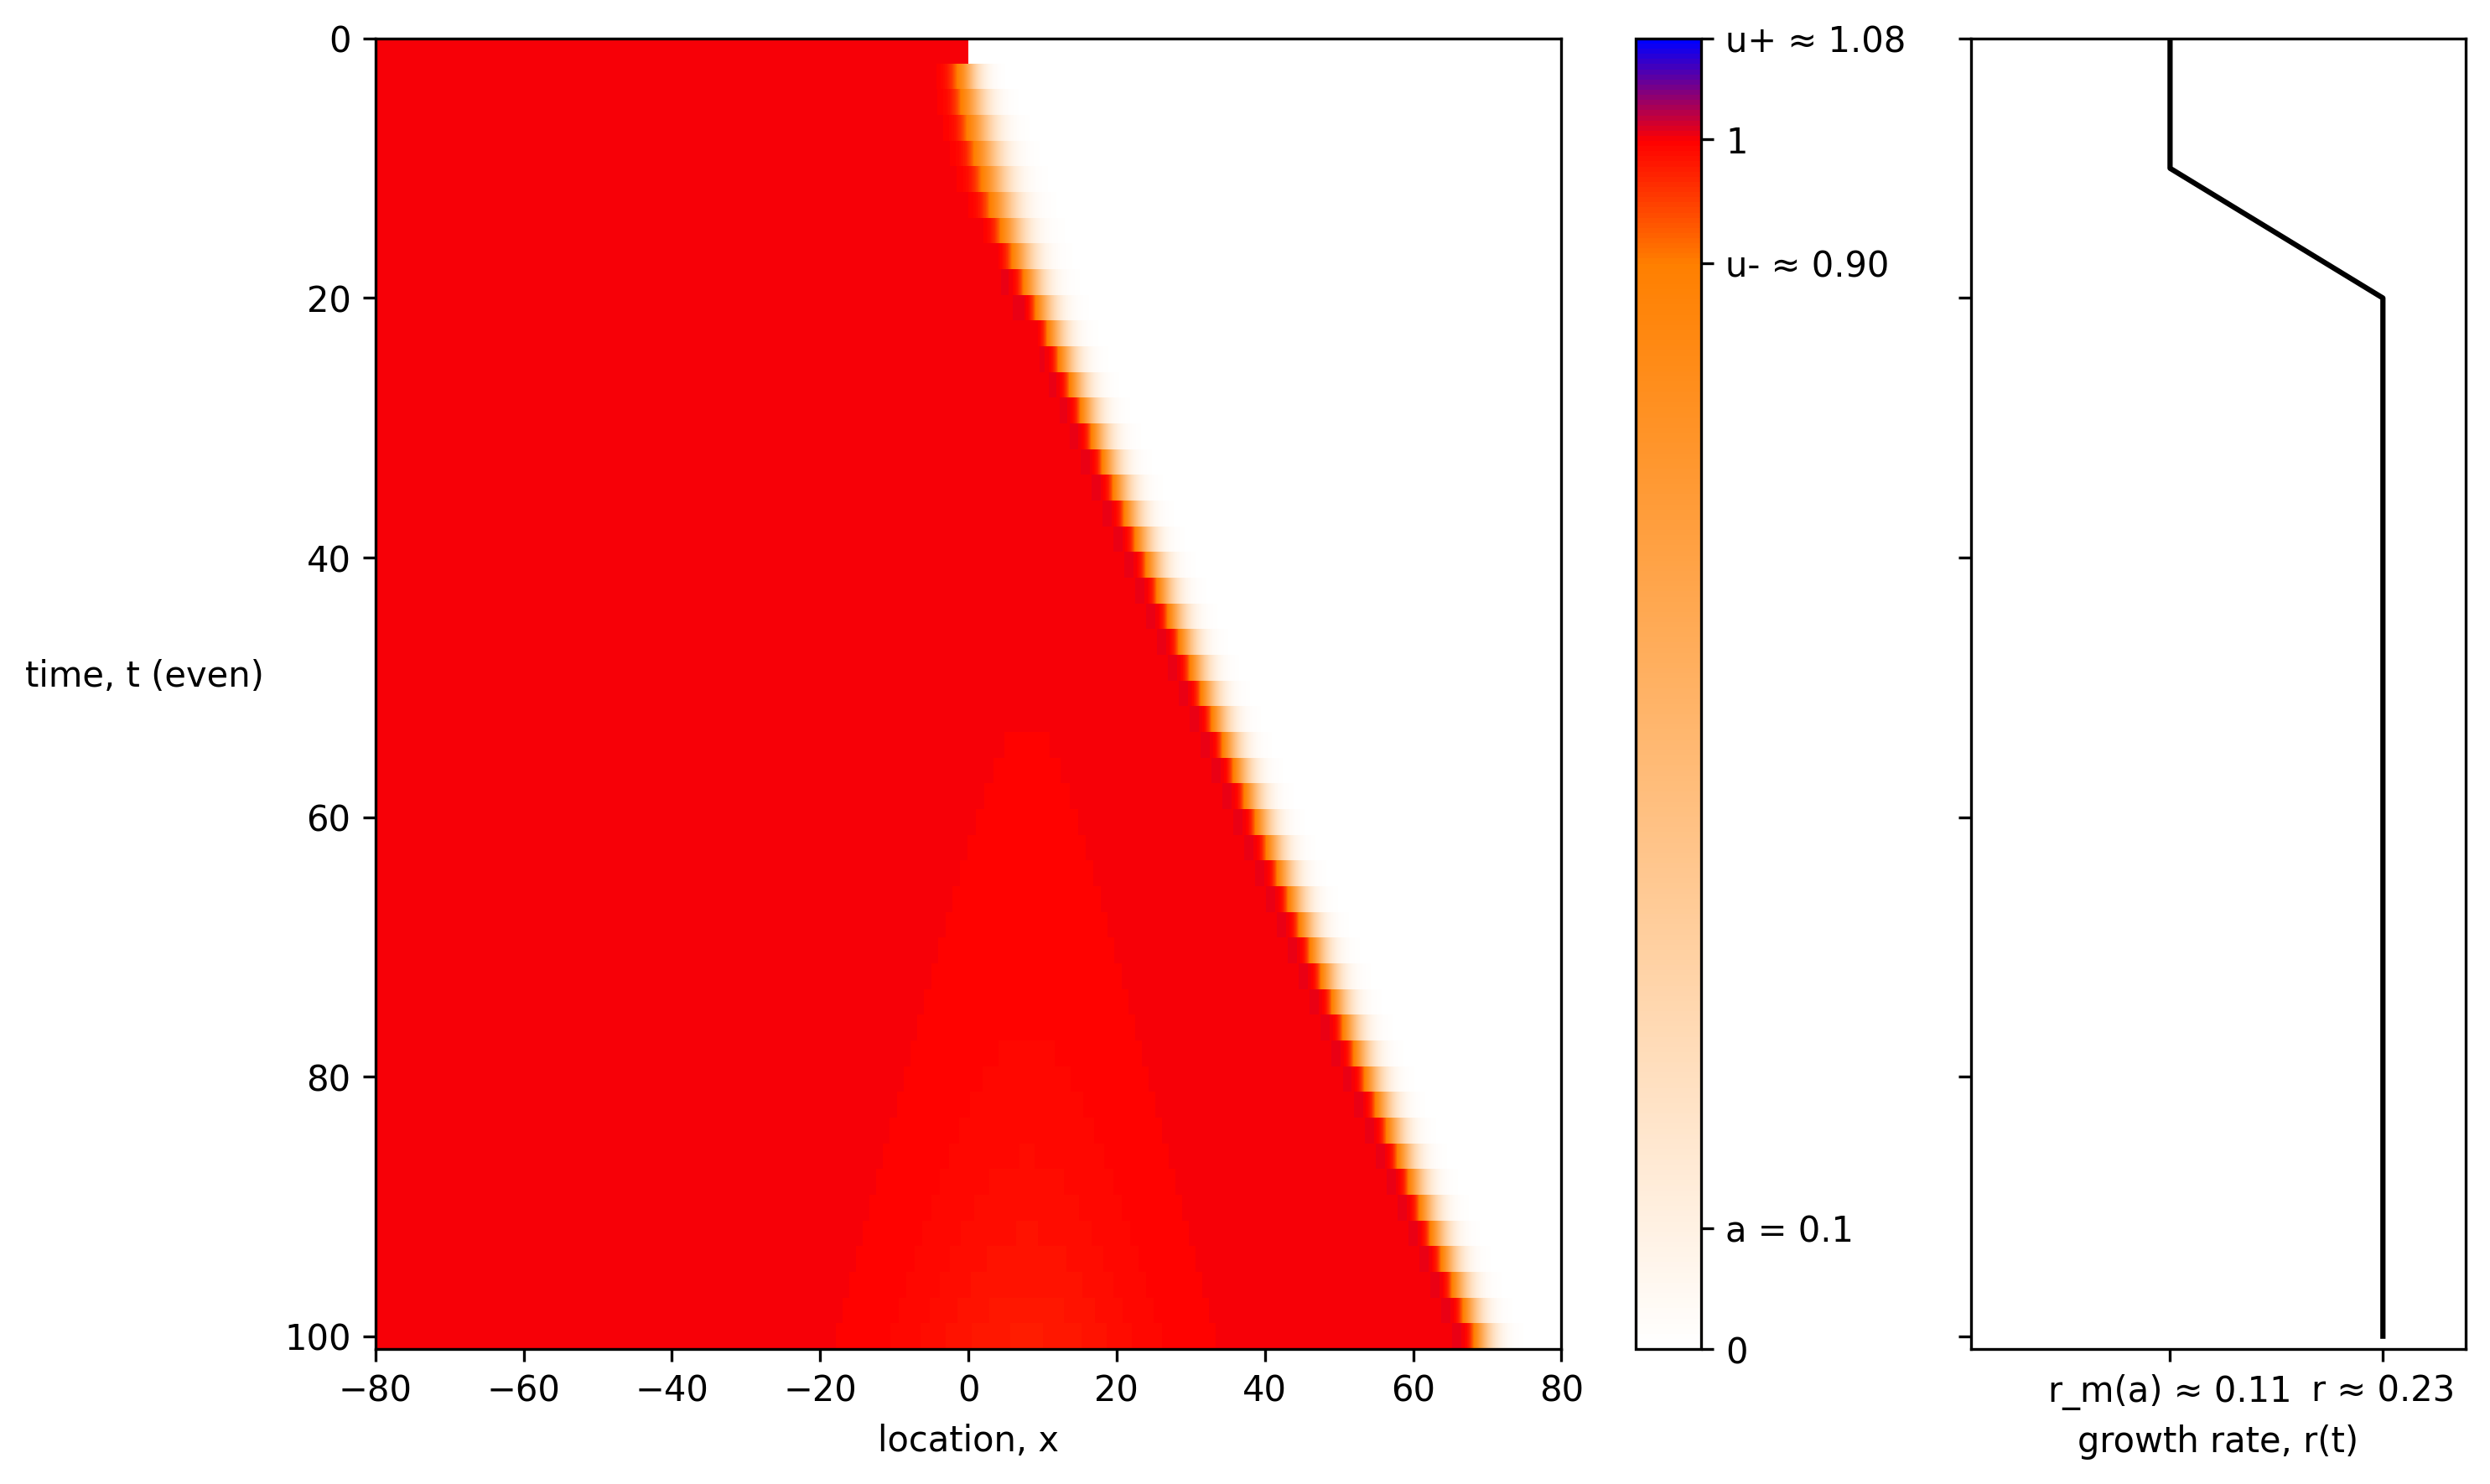
\includegraphics[width=0.5\textwidth]{figures/continuation_with_r.png}
    %\caption{The growth map with a couple different choices of parameters.}
    \label{fig:continuation}
\end{figure}

\subsection{Detecting dynamical stabilization}



\subsection{Main conjecture}



Our main conjecture is the following:

\begin{conjecture}

\end{conjecture}

% include the numerical plots here..

\section{Appendix}

\subsection{Traveling waves and stacked waves}

In this section we comment on the analytical interpretation of so-called `wave-train' solutions, aka stacked traveling waves or terraces.

Recall some basic facts about traveling waves:
\begin{enumerate}
\item A solution $u_t(x)$ is called a traveling wave with (rightward) velocity $c$ if it satisfies $$ u_{t+1}(x) = u_t(x-c) $$
Any traveling wave has the form
$$ u_t(x)=w(x-ct) $$
where $w$ is a solution to the equation
$$ Qw(x)=w(x-c) $$
We may call $w$ a traveling wave profile with velocity $c$.
\item A traveling front is a traveling waves with limits at $\pm \infty$, which are necessarily both fixed points of $g$, that is
$$ g(u_t(\pm\infty)) = u_t(\pm\infty) $$
\item A solution $u_t(x)$ is called a periodic traveling wave with period $p$ and mean velocity $c$ if it satisfies $$ u_{t+p}(x)=u_t(x-cp) $$
Any periodic traveling wave has the form
$$ u_t(x)=w_t(x-pc) $$
where $w$ solves the equation
$$ Q^pw_t(x)=w_t(x-pc) $$
and is periodic in $t$,
$$ w_{t+p}=w_t $$
We can say that $w_t$ is a periodic traveling wave profile.
\item A $p$-periodic traveling front is a $p$-periodic traveling wave with limits at $\pm\infty$, which are necessarily both $p$-periodic points of $g$, that is,
$$ g^p(u_t(\pm\infty)) = u_t(\pm\infty) $$
\item Alternatively we can just define a periodic traveling wave of $Q$ to be a traveling wave of $Q^p$.
\item We say that a solution $u_t(x)$ converges uniformly to a traveling wave if
$$ \lim_{t \to \infty} \sup_{x \in \mathbb{R}} |u_t(x)-w(x-c)| = 0 $$
where $w_t$ is a traveling wave profile with velocity $c$.
\item We say that a solution $u_t(x)$ converges uniformly to a periodic traveling wave if
$$ \lim_{t \to \infty} \sup_{x \in \mathbb{R}} |u_t(x)-w_t(x-pc)| = 0 $$
where $w_t$ is a periodic traveling wave profile with mean velocity $c$.
\end{enumerate}

It's not immediately clear how to adopt the above definitions to convergence to a stacked wave.

% \begin{proposition}
% Suppose $u_t(x)=w(x-c^*t)$ is a traveling wave solution with velocity $c^*$, and suppose $w$ has limits at $\pm\infty$ Then:
% \begin{enumerate}
% \item If $c<c^*$ then $u_t(x+ct) \to w(-\infty)$ uniformly on compact sets.
% \item If $c=c^*$ then $u_t(x+ct) \to w$ uniformly.
% \item If $c>c^*$ then $u_t(x+ct) \to w(+\infty)$ uniformly on compact sets.
% \end{enumerate}
% \begin{proof}
% \begin{enumerate}
% \item First assume $c<c^*$. Let $\epsilon>0$, let $K$ be a compact set, and let $R>0$ sufficiently large that $K \subseteq [-R,R]$. We want to show there exists $t_0$ such that $t \geq t_0$ implies $|u_t(x+ct)-w(-\infty)|<\epsilon$ for all $|x| \leq R$. We have
% $$ u_t(x+ct) = w(x+ct-c^*t)=w(x-(c^*-c)t) $$
% where $c^*-c$ is positive. By assumption, there exists $x_0$ such that $x \leq x_0$ implies $|w(x)-w(-\infty)|<\epsilon$. So it suffices to have
% $$ x-(c^*-c)t \leq x_0, \quad \forall |x| \leq R, \quad \forall t \geq t_0 $$
% For this it suffices to have
% $$ R-(c^*-c)t \leq x_0, \quad \forall t \geq t_0 $$
% Solving for $t$ it suffices to have
% $$ t \geq \frac{x_0-R}{c^*-c}, \quad \forall t \geq t_0 $$
% Hence take any $\displaystyle t_0 \geq \frac{x_0-R}{c^*-c}$ and the proof is complete.
% \item In the second case if $c=c^*$ then $u_t(x+ct)=w(x)$ so the difference is identically zero, so uniform convergence holds trivially.
% \item The third case mirrors the first case.
% \end{enumerate}
% \end{proof}
% \end{proposition}

% The next proposition strengthens the previous one:

\begin{proposition}
Suppose $u_t(x)$ converges to a traveling wave, that is
$$ \lim_{t\to\infty}\sup_{x \in \mathbb{R}}|u_t(x)-w(x-c^*t)|=0 $$
for some traveling wave profile $w$ with velocity $c^*$, and suppose $w$ has limits at $\pm\infty$ Then:
\begin{enumerate}
\item If $c<c^*$ then $u_t(x+ct) \to w(-\infty)$ uniformly on compact sets.
\item If $c=c^*$ then $u_t(x+ct) \to w$ uniformly.
\item If $c>c^*$ then $u_t(x+ct) \to w(+\infty)$ uniformly on compact sets.
\end{enumerate}
\begin{proof}
\begin{enumerate}
\item Suppose $c<c^*$ and let $K$ be a compact set. By the triangle inequality, for all $x$ and $t$,
$$ \begin{aligned}
\sup_{x \in K} |u_t(x+ct)-w(-\infty)| &\leq \sup_{x \in K} |u_t(x+ct)-w(x-(c^*-c)t)| \\
& + \sup_{x \in K}|w(x-(c^*-c)t)-w(-\infty)|
\end{aligned} $$
It suffices to show both terms on the right vanish as $t \to \infty$.

For the first term we have
$$ \begin{aligned} \sup_{x \in K} |u_t(x+ct)-w(x-(c^*-c)t)| &= \sup_{x \in (K+ct)}|u_t(x)-w(x-c^*t)| \\
&\leq \sup_{x \in \mathbb{R}}|u_t(x)-w(x-c^*t)|
\end{aligned} $$
which vanishes by assumption that $u_t$ converges to a traveling wave.

For the second part, $\epsilon>0$. We need to find $t_0$ such that 
$$ \sup_{x \in K}|w(x-(c^*-c)t)-w(-\infty)| < \epsilon, \quad \forall t \geq t_0$$
Let $x_0$ be such that $|w(x)-w(-\infty)|<\epsilon$ for all $x \leq x_0$. It suffices to choose $t_0$ such that
$$ x-(c^*-c)t \leq x_0, \quad \forall x \in K, \quad \forall t \geq t_0 $$
For this it suffices to have
$$ \sup K-(c^*-c)t \leq x_0, \quad \forall t \geq t_0 $$
Solving this inequality shows that it suffices to take any $\displaystyle t_0 \geq \frac{x_0-\sup K}{c^*-c}$.
\item If $c=c^*$ then simply apply translation inside the supremum:
$$ \lim_{t\to\infty} \sup_x |u_t(x+c^*t)-w(x)| = \lim_{t\to\infty} \sup_x |u_t(x)-w(x-c^*t)| = 0 $$
\item The third case mirrors the first case.
\end{enumerate}
\end{proof}
\end{proposition}

The next theorem generalizes this to periodic traveling waves.


\begin{remark}
The next proposition assumes $w_t$ has limits at $\pm\infty$ {\it uniformly in $t$}. This means:
$$
\forall \epsilon>0,\exists x_0,\forall t,\forall x\leq x_0,|w_t(x)-w_t(-\infty)|<\epsilon
$$
(and likewise at $+\infty$).
\end{remark}

\begin{proposition}
Suppose $u_t(x)$ converges to a periodic traveling wave, that is
$$ \lim_{t\to\infty}\sup_{x \in \mathbb{R}}|u_t(x)-w_t(x-c^*t)|=0 $$
for some periodic traveling wave profile $w_t$ with mean velocity $c^*$, and suppose $w_t$ has limits at $\pm\infty$ {\it uniformly in $t$}. Then:
\begin{enumerate}
\item If $c<c^*$ then $u_t(x+ct) \to w_t(-\infty)$ uniformly on compact sets.
\item If $c=c^*$ then $u_t(x+ct) \to w_t$ uniformly.
\item If $c>c^*$ then $u_t(x+ct) \to w_t(+\infty)$ uniformly on compact sets.
\end{enumerate}
Or if we want to be more precise:
\begin{enumerate}
\item If $c<c^*$ then $u_t(x+ct)-w_t(-\infty) \to 0$ uniformly on compact sets.
\item If $c=c^*$ then $u_t(x+ct)-w_t(x) \to 0$ uniformly.
\item If $c>c^*$ then $u_t(x+ct)-w_t(+\infty) \to 0$ uniformly on compact sets.
\end{enumerate}
\begin{proof}
\begin{enumerate}
\item Suppose $c<c^*$ and let $K$ be a compact set. By the triangle inequality, for all $x$ and $t$,
$$ \begin{aligned}
\sup_{x \in K} |u_t(x+ct)-w_t(-\infty)| &\leq \sup_{x \in K} |u_t(x+ct)-w_t(x-(c^*-c)t)| \\
& + \sup_{x \in K}|w_t(x-(c^*-c)t)-w_t(-\infty)|
\end{aligned} $$
It suffices to show both terms on the right vanish as $t \to \infty$.

For the first term we have
$$ \begin{aligned} \sup_{x \in K} |u_t(x+ct)-w_t(x-(c^*-c)t)| &= \sup_{x \in (K+ct)}|u_t(x)-w_t(x-c^*t)| \\
&\leq \sup_{x \in \mathbb{R}}|u_t(x)-w_t(x-c^*t)|
\end{aligned} $$
which vanishes as $t \to \infty$ by assumption that $u_t$ converges to a traveling wave.

For the second part, $\epsilon>0$. We need to find $t_0$ such that 
$$ \sup_{x \in K}|w_t(x-(c^*-c)t)-w_t(-\infty)| < \epsilon, \quad \forall t \geq t_0$$
Let $x_0$ be such that $|w_t(x)-w_t(-\infty)|<\epsilon$ for all $x \leq x_0$ and for all $t$. It suffices to choose $t_0$ such that
$$ x-(c^*-c)t \leq x_0, \quad \forall x \in K, \quad \forall t \geq t_0 $$
For this it suffices to have
$$ \sup K-(c^*-c)t \leq x_0, \quad \forall t \geq t_0 $$
Solving this inequality shows that it suffices to take any $\displaystyle t_0 \geq \frac{x_0-\sup K}{c^*-c}$.
\item If $c=c^*$ then simply apply translation inside the supremum:
$$ \lim_{t\to\infty} \sup_x |u_t(x+c^*t)-w_t(x)| = \lim_{t\to\infty} \sup_x |u_t(x)-w_t(x-c^*t)| = 0 $$
\item The third case mirrors the first case.
\end{enumerate}
\end{proof}
\end{proposition}

\subsection{Generalized defn}


\end{document}
